\clearpage
\section{Software Technology Stack}
\label{sec:technology}

\begin{center}
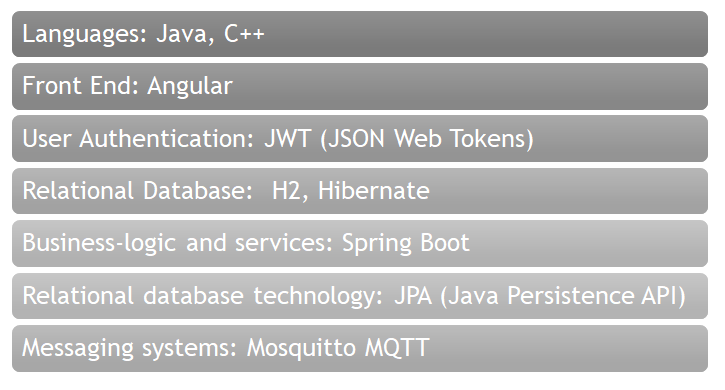
\includegraphics[scale=0.5]{figs/t_stack.png}
\par
Technology Stack
\end{center}

\subsection{Angular}
We chose Angular as our web application framework to develop the frontend of the FeedApp
prototype. Angular is a popular, open source TypeScript based framework\footnote{https://angular.io/guide/architecture } that is used to create
Single Page Applications (SPAs). SPAs are web applications that only loads one single page, and then
changes the content of that page depending on how the user interacts with the page.

\subsubsection{Fundamental Consepts of Angular }

\noindent Components: Components are many places described as the main building blocks for Angular applications. Each
component will contain one HTML-file with the UI-template of the component and one TypeScript-
file that contains the components logic. It can also contain CSS or SCSS files, defining the styles of the
component, as well as test files and configuration files. A component defines a specific view, as well
as the functionality that goes into that view. In other words, it contains both what the user sees in
the UI and the logic that goes into the component. \\

\noindent Services: It is also possible to share different functions and logic between different components. This
can be done by creating a service, which is a TypeScript file that is used for tasks such as for example
business logic and handling of data. In our FeedApp implementation, we created services dedicated to managing authentication and handling poll data. \\

\noindent Dependency Injection (DI): Services can also be used to inject dependencies into multiple
components, with the use of DI. This is useful for connecting the different parts of the application. \\

\noindent Routing: The Angular Router handles the navigation between different views as users performs different tasks. This is a key element in SPAs since instead of reloading the page every time the view is changed. \\

\noindent One of the main advantages of creating the application as a SPA is that it speeds up the development
process.


\subsection{Spring Boot}
\label{subsec:springboot}

We have chosen Spring Boot as our enterprice software framework when developing our application. Spring Boot is an extension of the Spring Framework that simplifies the development process, making it possible to create a functioning web application fast. Considering the time limitation we had on our project, Spring Boot seemed like a good choice when choosing a framework. 

\subsubsection{Spring Framework}

To fully understand the benefits of the Spring Boot extension, we are first going to briefly go through some core concepts in the Spring Framework\footnote{https://docs.spring.io/spring-framework/reference/index.html}:

\noindent Bean Definition: Beans are often described as the backbone of a Spring application. They are managed by the Spring Inversion of Control (IoC) Container. How they are configured, and how their lifecycle is managed plays an important role when having a smooth and proper running application. \\

\noindent Dependency Injection (DI): Spring's DI mechanism manages dependencies among application components. This setup is crucial for injecting required services and modules into different parts of the application. \\

\noindent Aspect-Oriented Programming (AOP): In Spring, AOP makes it possible to handle tasks that are common in multiple parts of an application efficiently by defining the function and then applying it to the sections that need to use it. \\


\noindent How a Spring application is deployed:

\begin{itemize}
    \item Packaging: The application is compiled and packaged, typically into a JAR or WAR file, ready for deployment.
    \item Running on a Server: The packaged application is deployed on a web server. Spring Boot, with its embedded server capability, simplifies this by allowing the application to run independently without needing a separate server setup.
\end{itemize}

\subsubsection{Spring Boot's Role in FeedApp:}

\noindent Auto-Configuration: Spring Boot automatically configures the application based on the included libraries, reducing the need for extensive manual configuration.\\

\noindent Simplified Deployment: The embedded server feature of Spring Boot allows our application to be deployed as a standalone unit, enhancing ease of deployment and portability.


\noindent In the implementation of our FeedApp prototype, the use of Spring Boots auto configuration and deployment functionalities has made it possible for us to spend more time on the applications business logic. 

\subsection{JSON Web Tokens}

\noindent We used an open standard called JSON Web Tokens (JWT), that provides a condensed, self-contained method for securely exchanging data as a JSON object between parties. This data is digitally signed, so it can be validated and trusted. RSA or ECDSA can be used to sign JWTs with a secret key or a public/private key pair. \footnote{https://datatracker.ietf.org/doc/html/rfc7519}\\

\noindent JWTs are essential to our FeedApp's authentication procedure. A JWT is given to a user upon login. Subsequent requests to authenticate the user and grant access to restricted routes, services, and resources within the application will then utilize this token. Because of their short size and ease of use, JWTs are the ideal format for our application and work well in our web-based environment.

\subsection{H2 Database}

\noindent We used a quick and easy approach to store and manage data with the lightweight H2 database. Because of its cheap overhead and ease of setup, it's especially helpful throughout the development and testing phases. H2 can operate embedded within a Java program or in client-server mode. \\

\noindent We are using the H2 database in FeedApp development for testing and prototyping. It eliminates the requirement for a complicated database setup and enables us to simulate database interactions and run unit tests. The H2 database is the perfect option for our needs for rapid development because it interfaces with our Spring Boot platform.


\subsection{Hibernate}

\noindent  For Java applications, Hibernate is a powerful Object-Relational Mapping (ORM) framework. It offers a framework for converting a conventional relational database to an object-oriented domain model. Hibernate resolves the mismatch issues by substituting high-level object handling routines with direct, permanent database accesses. \footnote{https://hibernate.org/orm/} \\

\noindent Hibernate is used in our FeedApp to make it easier for our Java application to communicate with the database. The CRUD (Create, Read, Update, Delete) procedures are made simpler and more effective by managing database operations and data persistence. Our team is able to concentrate more on the business logic and less on database management because Hibernate abstracts the database logic.

\subsection{Java Persistence API}

\noindent A Java specification for managing, retrieving, and storing data between Java objects and a relational database is called the Java Persistence API (JPA). JPA, which is a component of the Java EE platform, makes it easier to create Java apps that communicate with databases. \\

\noindent JPA is implemented into FeedApp to manage our application's relational data. It offers a platform for managing relational data in Java programs and executing database operations on Java Entities. Hibernate and JPA work together to make database administration in our application more error-free and efficient. \\


\subsection{Mosquitto MQTT}

\noindent A simple publish-subscribe network protocol called MQTT (Message Queuing Telemetry Transport) is used to send messages between devices. Mosquitto is portable and works with a wide range of devices, including powerful servers and single-board computers with minimal power consumption. \footnote{https://mosquitto.org/} \\

\noindent Mosquitto MQTT is essential to our FeedApp since it manages real-time messages and facilitates effective connectivity with IoT devices. MQTT is a good solution for our IoT-related capabilities since it guarantees efficient and reliable message delivery even in limited contexts. Maintaining the application's responsiveness and performance requires minimal resource usage, which is ensured by its lightweight design.



